\documentclass[11pt]{article}
\usepackage[dvipsnames]{xcolor}
\usepackage{times}
\usepackage{amsmath,amsthm,amssymb,setspace,enumitem,epsfig,titlesec,verbatim,array,eurosym,multirow}
\usepackage[sort&compress,numbers]{natbib}
\usepackage[footnotesize,bf]{caption}
\usepackage[margin=2.5cm, includefoot, footskip=30pt]{geometry}
\usepackage{standalone}
\usepackage{tikz}
\usepackage{subcaption}
\usepackage{hyperref}
\usepackage{tabularx}
\usepackage{booktabs}
\usepackage{blkarray}
\usepackage[ruled,vlined]{algorithm2e}
\smallskip % Erlaubt kleine Abstaende zwischen Paragraphen, falls es dem Seitenlayout hilft
\renewcommand{\baselinestretch}{1.15}
\usepackage{tikz}
\usetikzlibrary{arrows}
\usepackage{minitoc}
\usepackage{graphicx}
\usepackage{hyperref}
\usepackage{subcaption}
\usepackage{multirow}
\usepackage{multicol}
\usepackage{standalone}

\newcommand{\nikoleta}[1]{\textcolor{orange}{\textbf{NG}: #1}}
\newcommand{\christian}[1]{\textcolor{blue}{\textbf{CH}: #1}}

\newcommand{\figref}[1]{{\textbf{Fig.~\ref{#1}}}}

\def\wsls{\texttt{WSLS}}
\def\tft{\texttt{TFT}}
\def\tftt{\texttt{TF2T}}
\def\ttft{\texttt{2TFT}}
\def\gtft{\texttt{GTFT}}
\def\allc{\texttt{ALLC}}
\def\alld{\texttt{ALLD}}
\def\alt{\texttt{Alternator}}
\def\SI{\textbf{Supporting Information}}
\def\methods{\textbf{Material and Methods}}


\titleformat{\section}{\sffamily \fontsize{12}{15}\bfseries}{\thesection}{0.4em}{}
\titleformat{\subsection}{\sffamily\fontsize{11}{15}\bfseries}{\thesubsection}{0.4em}{}




\title{\bfseries \sffamily \Large Conditional cooperation with longer memory}

%% Perhaps: Better title (Conditional cooperation with longer memory) %% 

\author{Nikoleta E. Glynatsi$^{1,*}$, Martin A. Nowak$^2$, Christian Hilbe$^1$\\[0.3cm]
$^{\rm 1}$Max Planck Research Group on the Dynamics of Social Behavior,\\ Max Planck Institute for Evolutionary Biology, Pl\"{o}n, Germany \\
$^{\rm 2}$Department of Mathematics,
Department of Organismic and Evolutionary Biology,\\ Harvard University, Cambridge, USA\\
$^*$To whom correspondence should be addressed. E-mail: glynatsi@evolbio.mpg.de
}
\date{}

\begin{document}

\maketitle

~\\[0.5cm]
\noindent
{\bf 
Direct reciprocity is a wide-spread mechanism for evolution of cooperation. In
repeated interactions, players can condition their behavior on previous
outcomes. A well known approach is given by reactive strategies, which respond
to the co-player's previous move. Here we extend reactive strategies to longer
memories. A reactive-$n$ strategy takes into account the sequence of the last $n$
moves of the co-player. A reactive-$n$ counting strategy records how often the
co-player has cooperated during the last $n$ rounds. We derive an algorithm to
identify all partner strategies among reactive-$n$ strategies. We give explicit
conditions for all partner strategies among reactive-2, reactive-3 strategies,
and reactive-$n$ counting strategies. Partner strategies are those that ensure
mutual cooperation without exploitation. We perform evolutionary simulations and
find that longer memory increases the average cooperation rate for reactive-$n$
strategies but not for reactive counting strategies. Paying attention to the
sequence of moves is necessary for reaping the advantages of longer memory.
}\\[1cm]




\noindent
{\it Keywords:} Evolutionary game theory, direct reciprocity, evolution of cooperation, prisoner's dilemma

\clearpage
\newpage


%%%%%%%%%%%%%
%% SIGNIFICANCE  %%
%%%%%%%%%%%%%

\noindent
{\bf Significance statement.}
In repeated interactions, people tend to cooperate conditionally. They are
influenced by whether others cooperate with them, and react accordingly. Direct
reciprocity is based on repeated interactions between two players. Nice
strategies are those that are never the first to defect. Consequently, they
never seek to exploit the other. Partner strategies are nice strategies which
can sustain full cooperation as a Nash equilibrium. If you interact with such a
partner then you maximize your own payoff by full cooperation. Therefore,
partners resolve social dilemmas. Here we characterize all nice and all partner
strategies among longer memory reactive strategies. Our results show that
natural selection chooses partners. It pays to be nice.


%%%%%%%%%%%%%%
%%  INTRODUCTION  %%
%%%%%%%%%%%%%%

\section*{Introduction}

To a considerable extent, human cooperative behavior is governed by direct reciprocity~\cite{melis:ptrs:2010,rand:TCS:2013}. 
This mechanism for cooperation can explain why people return favors~\citep{neilson:JEBO:1999}, why they show more effort in group tasks when others do~\citep{fischbacher:AER:2010}, or why they stop cooperating when they feel exploited~\citep{hilbe:ncomms:2014,Xu:NComms:2016}. 
The main theoretical framework to describe reciprocity is the repeated prisoner's dilemma~\cite{axelrod:AAAS:1981, nowak:Science:2006, sigmund2010,Garcia:FRAI:2018,hilbe:Nature:2018,Rossetti:ETH:2023}. 
This game considers two individuals, referred to as players, who repeatedly decide whether to cooperate or to defect with one another~(\figref{fig:conceptual_figure_model}\textbf{A}). 
Both players prefer mutual cooperation to mutual defection. 
Yet given the co-player's action, each player has an incentive to defect. 
One common implementation of the prisoner's dilemma is the donation game. 
Here, cooperation simply means to pay a cost $c\!>\!0$ for the co-player to get a benefit $b\!>\!c$. 
Despite the simplicity of these games, they can give rise to remarkable dynamical patterns. 
These patterns have been explored in numerous studies~\citep{frean:PRSB:1994,killingback:PRSB:1999,hauert:JTB:2002b,kurokawa:PRSB:2009,pinheiro:PLoSCB:2014,garcia:jet:2016,mcavoy:PRSA:2019,Kraines:TaD:1989,nowak:Nature:1993,imhof:PNAS:2005,grujic:jtb:2012,van-segbroeck:prl:2012,press:PNAS:2012,stewart:pnas:2013,Toupo:IJBC:2014,stewart:pnas:2014, akin:EGADS:2016,glynatsi:scientific:2020,chen:PNASnexus:2023}.
Some of this literature describes how the evolution of cooperation depends on the game parameters, such as the benefit of cooperation, or the frequency with which errors occur~\citep{boyd:JTB:1989,Hao:PRE:2015,Zhang:GEB:2018,Mamiya:PRE:2020}. 
Others describe the effect of different learning dynamics~\citep{stewart:games:2015,Mcavoy:PNAS:2022}, of population structure~\citep{brauchli:JTB:1999,szabo:PRE:2000b,allen:AmNat:2013,szolnoki:scirep:2014}, or of the strategies that players are permitted to use~\citep{baek:scientific:2016}.  

Strategies of the repeated prisoner's dilemma can vary in their complexity.
While some are straightforward to implement, like always defect, many others are more sophisticated~\cite{harper:PLOSONE:2017, knight:PLOSONE:2018}.
To quantify a strategy's complexity, it is common to resort to the number of past rounds that the player needs to remember. 
Unconditional strategies like `always defect' or `always cooperate' are said to be \mbox{memory-0}. 
Strategies that only depend on the previous round, such as `Tit-for-Tat'~~\cite{axelrod:AAAS:1981,Duersch:IJGT:2013} or `Win-Stay Lose-Shift'~\cite{Kraines:TaD:1989,nowak:Nature:1993}, are \mbox{memory-1}~~(\figref{fig:conceptual_figure_model}\textbf{B}). 
Similarly, one can distinguish strategies that require more than one round of memory, or strategies that cannot be implemented with finite memory~\cite{Garcia:FRAI:2018}. 

Traditionally, most theoretical research on the evolution of reciprocity focuses on memory-1 strategies~\citep{nowak:Nature:1993,imhof:PNAS:2005,grujic:jtb:2012,van-segbroeck:prl:2012,press:PNAS:2012,stewart:pnas:2013,Toupo:IJBC:2014,stewart:pnas:2014, akin:EGADS:2016,glynatsi:scientific:2020,chen:PNASnexus:2023}. 
Although one-round memory can explain some of the empirical regularities in human behavior~\cite{engle:ET:2006, dal:AER:2011, camera:GEB:2012, bruttel:TD:2012,Montero-Porras:SciRep:2022},  people often take into account more than the last round~\cite{romero:EER:2018}.
Longer memory seems particularly relevant for noisy games, where people occasionally defect because of unintended errors~\cite{fudenberg:AER:2012}. 
However, a formal analysis of strategies with more than one-round memory has been difficult for two reasons. 
First, as the memory length $n$ increases, strategies become harder to interpret. 
For example, because two consecutive rounds of the prisoner's dilemma allow for 16 possible outcomes, memory-2 strategies need to specify 16 conditional cooperation probabilities~\citep{hauert:PRSB:1997}. 
Although some of the resulting strategies have an intuitive interpretation, such as `Tit-for-Two-Tat'~\citep{axelrod:AAAS:1981}, many others are difficult to make sense of. 
Second, the number of strategies, and the time it takes to compute their payoffs, increases dramatically in $n$. 
For example, for memory-1, there are $2^4\!=\!16$ deterministic strategies (strategies that do not randomize between different actions). 
When both players adopt memory-1 strategies, computing their payoffs requires the inversion of a $4\!\times\!4$ matrix~\cite{sigmund2010}. 
After increasing the memory length to memory-2, there are $2^{16}\!=\!64,536$ deterministic strategies, and payoffs now require the inverse of a $16\!\times\!16$ matrix. 
Probably for these reasons, previous studies considered simulations for small $n$~\citep{hauert:PRSB:1997,stewart:scientific:2016,Murase:PLoSCompBio:2023a}, or they analyzed the properties of a few selected higher-memory strategies~\citep{hilbe:PNAS:2017,ueda:RSOP:2021,li:NatureCompSci:2022}. 

To make progress, we focus on an easy-to-interpret subset of memory-$n$ strategies, the {\it reactive}-$n$ strategies. 
Capturing the basic premise of conditional cooperation, they only depend on the {\it co-player's} actions during the last $n$ rounds~(\figref{fig:conceptual_figure_model}\textbf{C,E}). 
While it has been difficult to explicitly characterize all Nash equilibria among the memory-$n$ strategies, we show that such a characterization is possible for reactive-$n$ strategies. 
Our results rely on a central insight, motivated by previous work by Press~\&~Dyson~\citep{press:PNAS:2012}: 
if one player adopts a reactive-$n$ strategy, the other player can always find a best response among the deterministic {\it self-reactive}-$n$ strategies. 
Self-reactive-$n$ strategies are remarkably simple. 
They only depend on the player's own previous $n$ moves (\figref{fig:conceptual_figure_model}\textbf{D,F}).
Based on this insight, we study all reactive-$n$ strategies that sustain full cooperation in a Nash equilibrium (the so-called {\it partner strategies}). 
We provide a full characterization for $n\!=\!2$ and $n\!=\!3$.
Even stronger results are feasible when we restrict attention to so-called {\it counting strategies}.  
Such strategies only react to how often the co-player has cooperated in the last $n$ rounds (irrespective of the exact timing of cooperation). 
For the donation game, we characterize the partners among the counting strategies for arbitrary~$n$. 
The resulting conditions are straightforward to interpret:
For every defection of the co-player in memory, the focal player's cooperation rate needs to drop by $c/(nb)$.
To further assess the relevance of partner strategies for the evolution of cooperation, we conduct extensive simulations for $n\!\in\!\{1,2,3\}$. 
Our findings indicate that the evolutionary process strongly favors partner strategies, and that these strategies are crucial for cooperation. 

Overall, our results provide important insights into the logic of conditional cooperation when players have more than one-round memory. 
We show that partner strategies exist for all repeated prisoner's dilemmas and for all memory lengths. 
To be stable, however, these strategies need to be sufficiently responsive to the co-player's previous actions. 


%%%%%%%%%%
%% RESULTS  %%
%%%%%%%%%%


\section*{Results}

%%%%%%
% Model %
%%%%%%

\textbf{Model and notation.}
We consider a repeated game between two players, player~1 and player~2.
Each round, players can choose to cooperate ($C$) or to defect ($D$). 
If both players cooperate, they receive the reward~$R$, which exceeds the (punishment) payoff~$P$ for mutual defection. 
If only one player defects, the defector receives the temptation payoff~$T$, whereas the cooperator ends up with the sucker's payoff~$S$. 
We assume payoffs satisfy the typical relationships of a prisoner's dilemma, $T \!>\! R \!>\! P \!>\! S$ and $2 R \!>\! T \!+\! S$. 
Therefore, in each round, mutual cooperation is the best outcome for the pair, but players have some incentive to defect. 
The players' aim is to maximize their average payoff per round, across infinitely many rounds.
To make results easier to interpret, it is sometimes instructive to look at a particular variant of the prisoner's dilemma, the donation game. 
Here, cooperation means to pay a cost $c\!>\!0$ for the co-player to get a benefit $b\!>\!c$.
The resulting payoffs are \(R \!\!=\! b\! -\! c, S \!=\! -c, T \!=\! b, P\!
=\! 0\). 
To illustrate our results, we focus on the donation game in the following. 
However, most of our findings are straightforward to extend to the general prisoner's dilemma (or to other repeated $2\!\times\!2$ games, see \SI). 

We consider players who use strategies with finite memory. 
To describe such strategies formally, we introduce some notation. 
The last $n$ actions of each player  $i\! \in\! \{1, 2\}$ are referred to as the player's {\it $n$-history}. 
We write this $n$-history as a tuple $\mathbf{h}^i\!=\!(a^i_{-n},\ldots,a^i_{-1})\!\in\!\{C,D\}^n$. 
Each entry $a^i_{-k}$ corresponds to player $i$'s action $k$ rounds ago. 
We use $H^i$ for the set of all such $n$-histories. 
This set contains $|H^i|\!=\!2^{n}$ elements. 
Based on this notation, we can define a {\it reactive}-$n$ {\it strategy} for player 1 as a vector $\mathbf{p}\!=\!(p_\mathbf{h})_{\mathbf{h}\in H^2} \!\in\! [0, 1]^{2^n}$. 
The entries $p_\mathbf{h}$ correspond to player 1's cooperation probability in any given round, contingent on player 2's actions during the last $n$ rounds. 
The strategy is called pure or deterministic if any entry is either zero or one. 
We note that the above definition leaves player 1's moves during the first $n$ rounds unspecified. 
However, in infinitely repeated games without discounting, these initial moves tend to be inconsequential. 
Hence, we neglect them in the following.

For \(n\!=\!1\), the above definition recovers the classical format of reactive-1 strategies~\cite{sigmund2010}, \(\mathbf{p}\!=\!(p_C, p_D)\). 
Here, $p_C$ and $p_D$ are the player's cooperation probability given that the co-player cooperated or defected in the previous round, respectively. 
This set contains, for example, the strategies of unconditional defection, \alld~$=\!(0,0)$, and Tit-for-Tat, \tft~$=\!(1,0)$. 
The next complexity class is the set of reactive-2 strategies, $\mathbf{p}\!=\!(p_{CC},p_{CD},p_{DC},p_{DD})$.
In addition to \alld{} and \tft{}, this set contains, for instance, the strategies Tit-for-Two-Tat, \tftt~$=\!(1,1,1,0)$ and Two-Tit-for-Tat,~\ttft$=\!(1,0,0,0)$. 
Similar examples exist for $n\!>\!2$. 
When both players adopt reactive-$n$ strategies (or more generally, memory-$n$ strategies), it is straightforward to compute their expected payoffs, by representing the game as a Markov chain. 
The respective procedure is described in the \SI{}.  

Herein, we are particularly interested in those reactive-$n$ strategies that sustain full cooperation. 
Such strategies ought to have two properties. 
First, they ought to be {\it nice}, meaning that they are never the first to defect~\citep{axelrod:AAAS:1981}.
This property ensures that two players with nice strategies fully cooperate. 
In particular, if $\mathbf{h}_C$ is a co-player's $n$-history that consists of $n$ bits of cooperation, a nice strategy needs to respond by cooperating with certainty, $p_{\mathbf{h}_C}\!=\!1$.  
Second, the strategy ought to form a {\it Nash equilibrium}, such that no co-player has an incentive to deviate. 
Strategies that have both properties are called {\it partner strategies}~\citep{Hilbe:GEB:2015} or {\it partners}.
The partners among the reactive-1 strategies are well known. 
For the donation game, partners are those strategies with $p_C\!=\!1$ and $p_D\!\le\!1\!-\!c/b$~\citep{akin:EGADS:2016}. 
However, a general theory of partners for $n\!\ge\!2$ is lacking. 
This is what we aim to derive in the following. 
In the main text, we provide the main intuition for our results; all proofs are in the \SI.\\
 
 
 
 %%%%%%%%
 %  Algorithm  %
 %%%%%%%%
 
\noindent
\textbf{An algorithm to identify partners among the reactive-$n$ strategies.} 
It is comparably easy to verify whether a reactive-$n$ strategy $\mathbf{p}$ is nice. 
Demonstrating that the strategy is also a Nash equilibrium, however, is far less trivial. 
In principle, this requires uncountably many payoff comparisons. 
We would have to show that if player 2's strategy is fixed to $\mathbf{p}$, no other strategy $\sigma$ for player~1 can result in a higher payoff. That is, player 1's payoff needs to satisfy $\pi^1(\sigma,\mathbf{p})\!\le\!\pi^1(\mathbf{p},\mathbf{p})$ for all $\sigma$. 
Fortunately, this task can be simplified considerably. 
Already Press~\& Dyson~\cite{press:PNAS:2012} showed that it is sufficient to test only those $\sigma$ with at most $n$ rounds of memory. 
Based on two insights, we can even further restrict the search space of strategies $\sigma$ that need to be tested.

First, suppose player~1 uses some arbitrary strategy $\sigma$ against player~2 with reactive-$n$ strategy \mbox{$\mathbf{p}\!=\!(p_\mathbf{h})_{\mathbf{h}\in H^1}$}. 
Then we prove that instead of $\sigma$, player~1 may switch to a {\it self-reactive}-$n$ strategy $\mathbf{\tilde{p}}$ without changing either player's payoffs. 
When adopting a self-reactive strategy, player~1 only takes into account her own actions during the last $n$ rounds, 
$\mathbf{\tilde{p}} \!=\! (\tilde{p}_\mathbf{h})_{\mathbf{h} \in H^1}$.
In particular, if $\sigma$ is a best response to $\mathbf{p}$, then there is an associated self-reactive strategy $\mathbf{\tilde p}$ that is also a best response. 
This result follows the same intuition as a similar result of Press \& Dyson~\cite{press:PNAS:2012}: 
if there is a part of the joint history that player~2 does not take into account, player~1 gains nothing by considering that part of the history. 
In our case, because player~2 only considers the last $n$ actions of player~1, it is sufficient for player~1 to do the same.
\figref{fig:conceptual_figure_results}\textbf{A,B} provides an illustration.  
There, we depict a game in which player~1 adopts a memory-1 strategy against a reactive-1 opponent. 
Due to the above result, we can find an equivalent self-reactive-1 strategy for player~1. 
While that self-reactive strategy is simpler, on average it induces the same game dynamics. 
Hence, it results in identical payoffs. 

The above result guarantees that for any reactive-$n$ strategy, there is always a best response among the self-reactive-$n$ strategies. 
In a second step, we prove that such a best response can always be found among the {\it deterministic} self-reactive-$n$ strategies. 
This reduces the search space for potential best responses further, from an uncountable set to a finite set of size $2^{2^n}$. 
For $n\!=\!2$, this leaves us with 16 self-reactive strategies to test. 
For $n\!=\!3$, we end up with (at most) 256 strategies. 
While this may still appear to be a large number, many of the different strategies impose redundant constraints on partner strategies.
This redundancy further reduces the number of conditions a partner needs to satisfy.\\


%%%%%%%%%%%%
% Partners for n=2,3  %
%%%%%%%%%%%%

\noindent
\textbf{Partners among the reactive-2 and the reactive-3 strategies.}
To illustrate the above algorithm, we first characterize the partners among the reactive-$2$ strategies. 
To this end, we note that it is straightforward to compute the payoff of a specific self-reactive-2 strategy against a general reactive-2 strategy $\mathbf{p}$ (see \SI{} for details). 
By computing the payoffs of all 16 pure self-deterministic strategies $\mathbf{\tilde p}$, and by requiring $\pi^1(\mathbf{\tilde p},\mathbf{p}) \!\le\! \pi^1(\mathbf{p},\mathbf{p})$ for all of them, we end up with only three conditions. Specifically, we prove that $\mathbf{p}$ is a partner if and only if
\begin{equation}\label{eq:two_bit_conditions}
  p_{CC} = 1, \qquad  \frac{p_{CD} + p_{DC}}{2} \le 1 - \frac{1}{2} \!\cdot\! \frac{c}{b}, \qquad  p_{DD} \leq 1\!-\! \frac{c}{b}.
\end{equation}
The above conditions define a three-dimensional polyhedron within the space of all nice reactive-2 strategies~(\figref{fig:conceptual_figure_results}\textbf{C}).
%These conditions are straightforward to interpret. 
The condition $p_{CC}\!=\!1$ follows from the requirement that the strategy ought to be nice. 
As long as the co-player cooperates, the reactive-$n$ player goes along. 
The other two conditions imply that for each defection in memory, the player's cooperation rate decreases by $c/(2b)$.
Interestingly, in cases with a mixed $2$-history (one cooperation, one defection), the above conditions suggest that the exact timing of cooperation does not matter. 
It is only required that the two cooperation probabilities $p_{CD}$ and $p_{DC}$ are sufficiently small {\it on average}. 
Notably, the above conditions also imply that to check whether a given reactive-2 strategy is a partner, it suffices to check two deviations. 
These deviations are the strategy that strictly alternates between cooperation and defection (yielding the first inequality), and \alld~(yielding the second inequality) (\figref{fig:conceptual_figure_conditions}). 
We note that this last implication is specific to the donation game. 
For the general prisoner's dilemma (depicted in \figref{fig:conceptual_figure_results}\textbf{D}), there are more than two inequalities that need to be satisfied (see~\SI{}).

Analogously, we can also characterize the partners among the reactive-3 strategies. 
A reactive-3 strategy is defined by the vector 
$
\mathbf{p} = (p_{CCC},\, p_{CCD},\, p_{CDC},\, p_{CDD},\, p_{DCC},\, p_{DCD},\, p_{DDC},\, p_{DDD}).
$
It is a partner strategy if and only if
\begin{align}\label{eq:three_bit_conditions}
  \begin{split}
  p_{CCC} & = 1 \\[0.2cm]
  \frac{p_{CDC} + p_{DCD}}{2} & \leq 1 - \frac{1}{2} \cdot \frac{c}{b} \\[0.2cm]
  \frac{p_{CCD} + p_{CDC} + p_{DCC}}{3} & \leq 1 - \frac{1}{3} \cdot \frac{c}{b} \\[0.2cm]
  \frac{p_{CDD} + p_{DCD} + p_{DDC}}{3} & \leq 1 - \frac{2}{3} \cdot \frac{c}{b} \\[0.2cm]
  \frac{p_{CCD} + p_{CDD} + p_{DCC} + p_{DDC}}{4}  & \leq 1 - \frac{1}{2} \cdot \frac{c}{b}  \\[0.2cm]
  p_{DDD} & \leq 1\!-\! \frac{c}{b}
  \end{split}
\end{align}
These conditions follow a similar logic as in the previous case with $n\!=\!2$:
for every co-player's defection in memory, the respective cooperation
probability needs to be diminished proportionally. These conditions
conditions also imply that to check whether a given reactive-3 strategy is a
partner, it suffices to check five deviations. Similarly to the previous case,
two of these deviations include the strategy that strictly alternates between
cooperation and defection, and \alld. The rest of the conditions arise from
deviations towards sequence-playing self-reactive strategies, where the
sequences are \((CCD)\), \((DCC)\), and \((DDCC)\) (\figref{fig:conceptual_figure_conditions}).
For $n\!=\!3$, there are now more conditions to consider than in the previous
case, and these conditions become even more complex for the general prisoner's
dilemma. Given these complexities, we do not present conditions for reactive-$n$
partner strategies beyond $n\!=\!3$, even though the algorithm presented in the
previous section still applies.\\

%%%%%%%%%%%%%
%  Counting strategies  %
%%%%%%%%%%%%%

\noindent
\textbf{Partners among the reactive-$n$ counting strategies.}
We can more easily generalize these formulas to the case of arbitrary $n$ if we further restrict the strategy space. 
In the following, we consider reactive-$n$ {\it counting strategies}. 
These strategies take into account how often the co-player cooperated during the past $n$ rounds. 
However, they do not consider in which of the past $n$ rounds the co-player cooperated. 
In the following, we represent such strategies as a vector $\mathbf{r}\!=\!(r_i)_{i \in \{n, n -1, \dots, 0\}}$. 
Each entry \(r_i\) indicates the player's cooperation probability if the co-player cooperated \(i\) times during the last \(n\) rounds. 
Note that any reactive-1 strategy $\mathbf{p}\!=\!(p_{C}, p_{D})$ is a counting strategy by definition. 
However, for larger $n$, the set of counting strategies is a strict subset of the reactive-$n$ strategies.
For example, for $n\!=\!2$, counting strategies are those strategies that satisfy $p_{CD}\!=\!p_{DC}\!=:\!r_1$. 
As a result, the partners among the counting strategies form a 2-dimensional plane within the 3-dimensional polyhedron of reactive-2 partner strategies (\figref{fig:conceptual_figure_results}\textbf{C,D}).

For the donation game among players with counting strategies, it is possible to characterize the set of partner strategies for arbitrary $n$. We find that a counting strategy $\mathbf{r}$ is a partner if and only if
\begin{equation} \label{eq:counting}
  r_n = 1 \qquad \text{and} \qquad r_{n - k} \le 1\! -\! \frac{k}{n} \!\cdot\! \frac{c}{b}~~ \text{ for }~k \!\in\! \{1, 2, \dots, n\}.
\end{equation}
That is, for every defection of the opponent in memory, the maximum cooperation probability needs to be reduced by $c/(nb)$.
It is worth to highlight that this result is general. 
These strategies are Nash equilibria even if players are allowed to deviate towards strategies that do not merely count the co-player's cooperative acts, or towards strategies that take into account more than the last $n$ rounds.\\ 


%%%%%%%%%%%%%%%
% Evolutionary simulations  %
%%%%%%%%%%%%%%%

\noindent
\textbf{Evolutionary Dynamics.}
With our previous equilibrium analysis we have identified the strategies that can sustain cooperation in principle. 
In a next step, we determine whether these strategies can evolve in the first place. 
Here, we no longer presume that individuals would play equilibrium strategies. 
Rather they initially implement some random behavior. 
Over time, however, they adapt their strategies based on social learning.
To model this learning process, we consider a population of individuals who update their strategies based on pairwise comparisons. 
The efficacy of the resulting learning process is determined by a strength of selection parameter~$\beta$. 
The larger $\beta$, the more likely individuals imitate strategies with a higher payoff. 
In addition, mutations occasionally introduce new strategies.
We describe the exact setup of this learning process in the \methods{} section.
As we explain there, the process is particularly easy to explore when mutations are rare~\cite{fudenberg:JET:2006,wu:JMB:2012,imhof:royal:2010,mcavoy:jet:2015}. 
In that case, the population is typically homogeneous, such that all players adopt the same (resident) strategy.   
Once a new mutant strategy appears, this strategy fixes or goes extinct before the next mutation happens. 
Evolutionary processes with rare mutations can be simulated more efficiently because there is an explicit formula for the mutant's fixation probability~\citep{nowak:Nature:2004}. 

The results of these simulations are shown in \figref{fig:evolutionary_results}. 
First, we explore which reactive-$n$ strategies evolve for a fixed set of game parameters. 
Here, we only vary the strategies' memory length $n$, and whether mutations can introduce all reactive-$n$ strategies, or counting strategies only. 
For ten independent simulations, \figref{fig:evolutionary_results}\textbf{A,B} displays the most abundant strategy for each simulation run (those are the strategies that prevent the largest number of mutants from taking over). 
We note that all the shown strategies show behavior consistent with our characterization of partners: 
If a co-player fully cooperated in the previous $n$ rounds, these strategies prescribe to continue with cooperation. 
If the co-player defected, however, they cooperate with a markedly reduced cooperation probability that satisfies the constraints in Eqs.~\eqref{eq:two_bit_conditions} -- \eqref{eq:counting}. 

In a next step, we systematically explore the impact of three key parameters: the cost-to-benefit ratio~$c/b$, the selection strength $\beta$, and the memory length~$n$. 
In each case, we record how these parameters affect the abundance of partner strategies and the population's average cooperation rate. 
Overall, the effect of each parameter is largely as expected~(\figref{fig:evolutionary_results}\textbf{C,D}).  
In particular, interactions are most cooperative when the cost-to-benefit ratio is small, such that cooperation is cheap. 
This effect is magnified for stronger selection strengths. 
Two results, however, are particularly noteworthy. 
First, the curves representing evolving cooperation rates align with the prevalence of partner strategies. 
This observation suggests that partner strategies are indeed crucial for the evolution of cooperation. 
Second, higher memory only has a notably positive effect on cooperation for reactive-$n$ strategies. 
In contrast, for counting strategies the effect of increasing $n$ is negligible. 
This observation highlights that the timing of cooperation is important, even in additive games such as the donation game. 


%%%%%%%%%%%%
%% DISCUSSION  %%
%%%%%%%%%%%%

\section*{Discussion}

Direct reciprocity is a key mechanism for cooperation, based on the intuition that individuals are more likely to cooperate when they meet repeatedly~\citep{nowak:Science:2006}.
To capture the logic of reciprocity, most previous theoretical studies focus on a subset of strategies, the  memory-1 strategies~\citep{nowak:Nature:1993,imhof:PNAS:2005,grujic:jtb:2012,van-segbroeck:prl:2012,press:PNAS:2012,stewart:pnas:2013,Toupo:IJBC:2014,stewart:pnas:2014, akin:EGADS:2016,glynatsi:scientific:2020,chen:PNASnexus:2023}. 
This set is comparably easy to work with: 
the number of deterministic memory-1 strategies is manageable; most strategies are easy to interpret; and payoffs can be computed efficiently~\citep{sigmund2010}. 
At the same time, however, this strategy space leaves out many interesting reciprocal behaviors that are of theoretical or empirical relevance.
For example, already simple behaviors such as Tit-for-Two-Tat~\citep{axelrod:AAAS:1981} are not representable with one-round memory.
This shortcoming is particularly consequential for noisy games, where higher-memory strategies are important~\cite{fudenberg:AER:2012}. 
In such games, individuals often take into account information from previous rounds to make sense of a co-player's defection in the last round. 
That is, the earlier history of play provides an important context to interpret the co-player's last-round behavior. 

To make progress, we consider an easily interpretable set of strategies with higher memory. 
These reactive-$n$ strategies take into account a co-player's moves during the past $n$ rounds. 
They capture the basic idea of conditional cooperation: people are responsive to the previous actions of their interaction partners. 
For reactive-$n$ strategies, we derive a convenient method to characterize all `partner strategies' -- strategies that sustain full cooperation in a Nash equilibrium~\citep{akin:EGADS:2016,Hilbe:GEB:2015}. 
We show that for a reactive-$n$ strategy to be a Nash equilibrium, it is not necessary to check all possible deviations. 
It suffices to only check deviations towards (deterministic) self-reactive-$n$ strategies. 
Self-reactive players are particularly simple to describe. 
They only take into account their own previous moves. 
In particular, the future behavior of a self-reactive player is independent of the co-player. 
We use this insight to characterize the reactive-$n$ partner strategies in the repeated prisoner's diemma.
But the same insight can be applied to other contexts. 
For example, it can be equally used to characterize other Nash equilibria (not only the cooperative ones). 
Similarly, it can be used to characterize the Nash equilibria of other repeated games, such as the snowdrift game~\citep{doebeli:EL:2005} or the volunteer's dilemma~\citep{diekmann:jcr:1985}.  
In this way, some of our technical results represent useful tools to make further progress on the theory of repeated games, similar to Press and Dyson's insight that any memory-1 strategy has a memory-1 best response~\citep{press:PNAS:2012}. 

Especially for small memory lengths, the conditions for partner strategies are intuitive. 
For example, for the donation game with $n\!=\!2$ rounds of memory, we end up with three conditions, see Eq.~\eqref{eq:two_bit_conditions}.
({\it i}) If the co-player cooperated twice, continue to cooperate; 
({\it ii}) If the co-player cooperated once, cooperate with a slightly reduced probability of $1\!-\!c/(2b)$ on average. 
({\it iii}) If the co-player did not cooperate at all, reduce the cooperation probability even further, to $1\!-\!c/b$. 
As we increase the memory length to $n\!\ge\!3$, or as we consider more general games, there are more conditions to satisfy, and the conditions become harder to interpret. 
However, the three simple conditions above do generalize to larger $n$ if we focus on the subset of counting strategies. 
These are the reactive-$n$ strategies that merely count how often the co-player cooperated during the last $n$ rounds. 
For counting strategies, we show that for each defection of the co-player in memory, a partner reduces its cooperation probability by $c/(nb)$. 
A partner's generosity decreases in proportion to their opponent's selfishness. 

With respect to {\it sustaining} cooperation, counting strategies thus seem to be just as effective as the more complex reactive-$n$ strategies.
With respect to the {\it evolution} of cooperation, however, they seem seem far less effective. 
In simulations, memory size only has a positive impact on evolving cooperation rates for reactive-$n$ strategies, but not for counting strategies~(\figref{fig:evolutionary_results}). 
These results suggest that memory is not only important to record {\it how often} a co-player cooperated, but also {\it when}. 
Overall, these results shed an important light on the logic of reciprocity for individuals with plausible cognitive abilities. 
While in practice, people's cooperative decisions often depend on the outcome of their last encounter, they rarely depend on that last encounter {\it only}. 
Our results suggest a way how individuals can integrate information from previous interactions to cooperate most effectively.  




%%%%%%%%%%
%% METHODS %%
%%%%%%%%%%

\subsection*{Materials and Methods}\label{section:materials_and_methods}

Our study combines two independent approaches, an equilibrium analysis and evolutionary simulations.\\

\noindent
{\bf Equilibrium analysis.} Here we only summarize our equilibrium analysis; all details are in the \SI. 
There, we formally introduce the three relevant strategy spaces, memory-$n$ strategies, reactive-$n$ strategies, and self-reactive-$n$ strategies. 
Then we provide an explicit algorithm for computing these strategies' payoffs. 
This algorithm uses a Markov chain approach. 
The states of the Markov chain are the possible combinations of $n$-histories of the two players. 
Given the players' current $n$-histories and their strategies, we can compute the likelihood of observing each possible state one round later. 

In a second step, we explore the partner strategies among the reactive-$n$ strategies. 
To this end, we first generalize some well-known reactive-1 partner strategies: Tit-for-Tat~\citep{axelrod:AAAS:1981} and Generous Tit-for-Tat~\citep{nowak:Nature:1992,molander:jcr:1985}. 
In a next step, we derive a general algorithm to check whether a given reactive-$n$ strategy is a partner. 
We use this algorithm to characterize all reactive-$n$ partners for $n\!\in\!\{1,2,3\}$, for both the donation game and the prisoner's dilemma. 
For counting strategies, we characterize the partners for all $n$.\\

\noindent
{\bf Evolutionary analysis.} For our simulations, we consider a population of size \(N\) where initially all
members are of the same strategy. 
In our case the initial population consists of unconditional defectors. 
In each elementary time step, one individual switches to a new mutant strategy. 
The mutant strategy is generated by randomly drawing cooperation probabilities from the unit interval \([0,1]^{2^n}\). 
If the mutant strategy yields a payoff of \(\pi_{M, k}\), where \(k\) is the number of
mutants in the population, and if residents get a payoff of \(\pi_{R,
k}\), then the fixation probability \(\phi_{M}\) of the mutant strategy can be
calculated explicitly~\citep{nowak:Nature:2004},
\begin{equation}\label{eq:fixation_probability}
  \phi_{M} =\Big(1 + \displaystyle \sum_{i=1}^{N - 1} \prod_{j=1}^{i} e^{- \beta (\pi_{M, j} - \pi_{R, i})} \Big)^{-1}.
\end{equation}
The parameter \(\beta \geq 0\) reflects the strength of selection. 
It measures the importance of relative payoff advantages for the evolutionary success of a strategy. 
When \(\beta\) is small, \(\beta \approx 0\), payoffs become irrelevant, and a strategy's fixation probability approaches
\(\phi_{M} \approx 1 / N\). 
The larger the value of \(\beta\), the more strongly the evolutionary process favors the fixation of strategies with a high
payoff.
Depending on \(\phi_{M}\), the mutant either fixes (becomes the new resident) or goes extinct. 
Afterwards, another mutant strategy is introduced to the population. 
We iterate this elementary population updating process for a large number of
mutant strategies. At each step, we record the current resident
strategy and the resulting average cooperation rate, indicating how often the
resident strategy cooperates with itself. Additionally, we assess how many
resident strategies qualify as partner strategies in our simulation. For a
resident strategy to be classified as a partner, it must satisfy all
inequalities in the respective definition of partner strategies and cooperate
with a probability of at least 95\% after full cooperation. 



\section*{Data, Materials, and Software Availability}

The source code used to reproduce the results of this study is available on the
online GitHub repository:
\href{https://github.com/Nikoleta-v3/conditional-cooperation-with-longer-memory}{Nikoleta-v3/conditional-cooperation-with-longer-memory}.
The simulation data have been archived on Zenodo and can be found at:
\href{https://zenodo.org/records/10605988}{zenodo.org/records/10605988}.

{\setlength{\bibsep}{0\baselineskip}
\bibliographystyle{naturemag}
\bibliography{bibliography.bib}
}


\clearpage
\newpage

\begin{figure}[t]
  \centering
  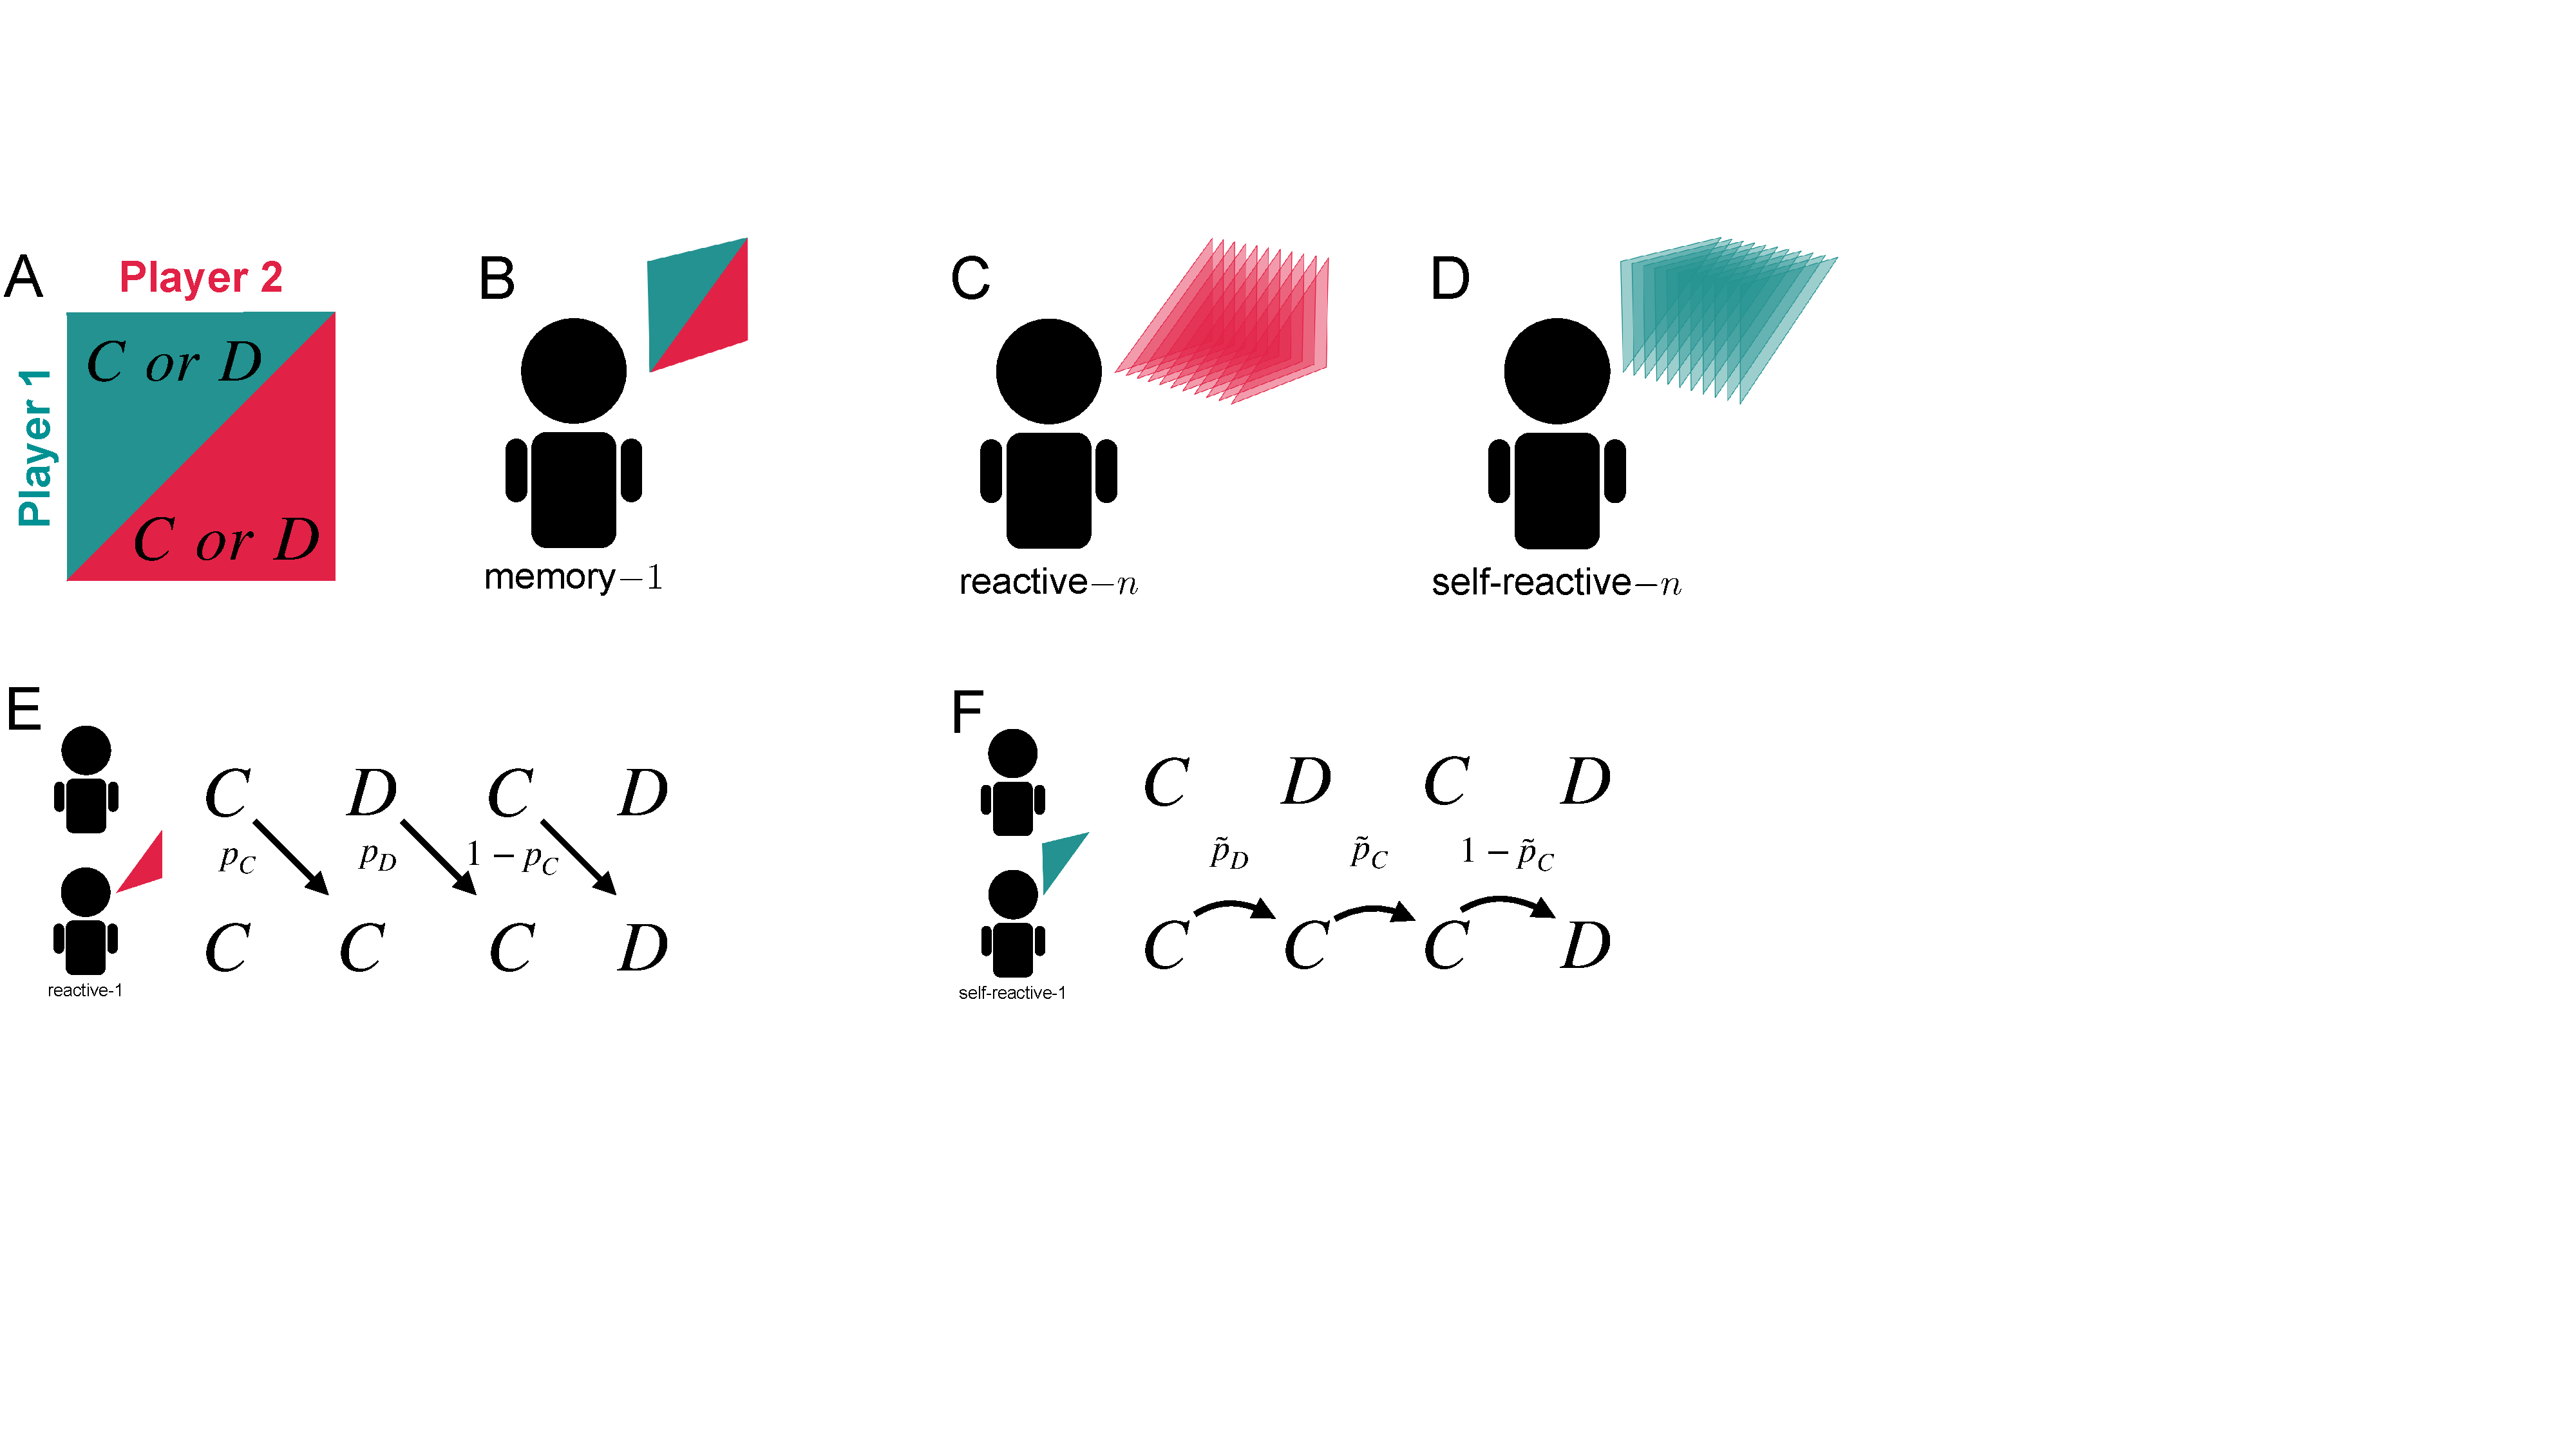
\includegraphics[width=0.75\textwidth]{figures/conceptual_figure.pdf}
  \caption{\textbf{The repeated prisoner's dilemma among players with finite memory.}
  \textbf{A,} In the repeated prisoner's dilemma, in each round two players independently decide whether to cooperate~($C$) or to defect~($D$). 
   \textbf{B,} When players adopt memory-1 strategies, their decisions depend on the entire outcome of the previous round. That is, they consider both their own and the co-player's previous action. 
   \textbf{C,} When players adopt a reactive-$n$ strategy, they make their decisions based on the co-player's actions during the past $n$ rounds. 
   \textbf{D,} A self-reactive-$n$ strategy is contingent on the player's own actions during the past $n$ rounds. 
   \textbf{E,} To illustrate these concepts, we show a game between a player with a reactive-$1$ strategy (top) and an arbitrary player (bottom). 
   Reactive-1 strategies can be represented as a vector  $\mathbf{p} \!=\! (p_C, p_D)$. 
   The entry $p_C$ is the probability of cooperating given the co-player cooperated in the previous round.
   The entry $p_D$ is the cooperation probability after the co-player defected. 
   \textbf{E,} Now, the top player adopts a self-reactive-1 strategy, $\mathbf{\tilde p}\!=\!(\tilde p_C, \tilde p_D)$. 
   Here, the bottom player's cooperation probabilities depend on their own previous action.
   }\label{fig:conceptual_figure_model}
\end{figure}


\begin{figure}[t]
  \centering
  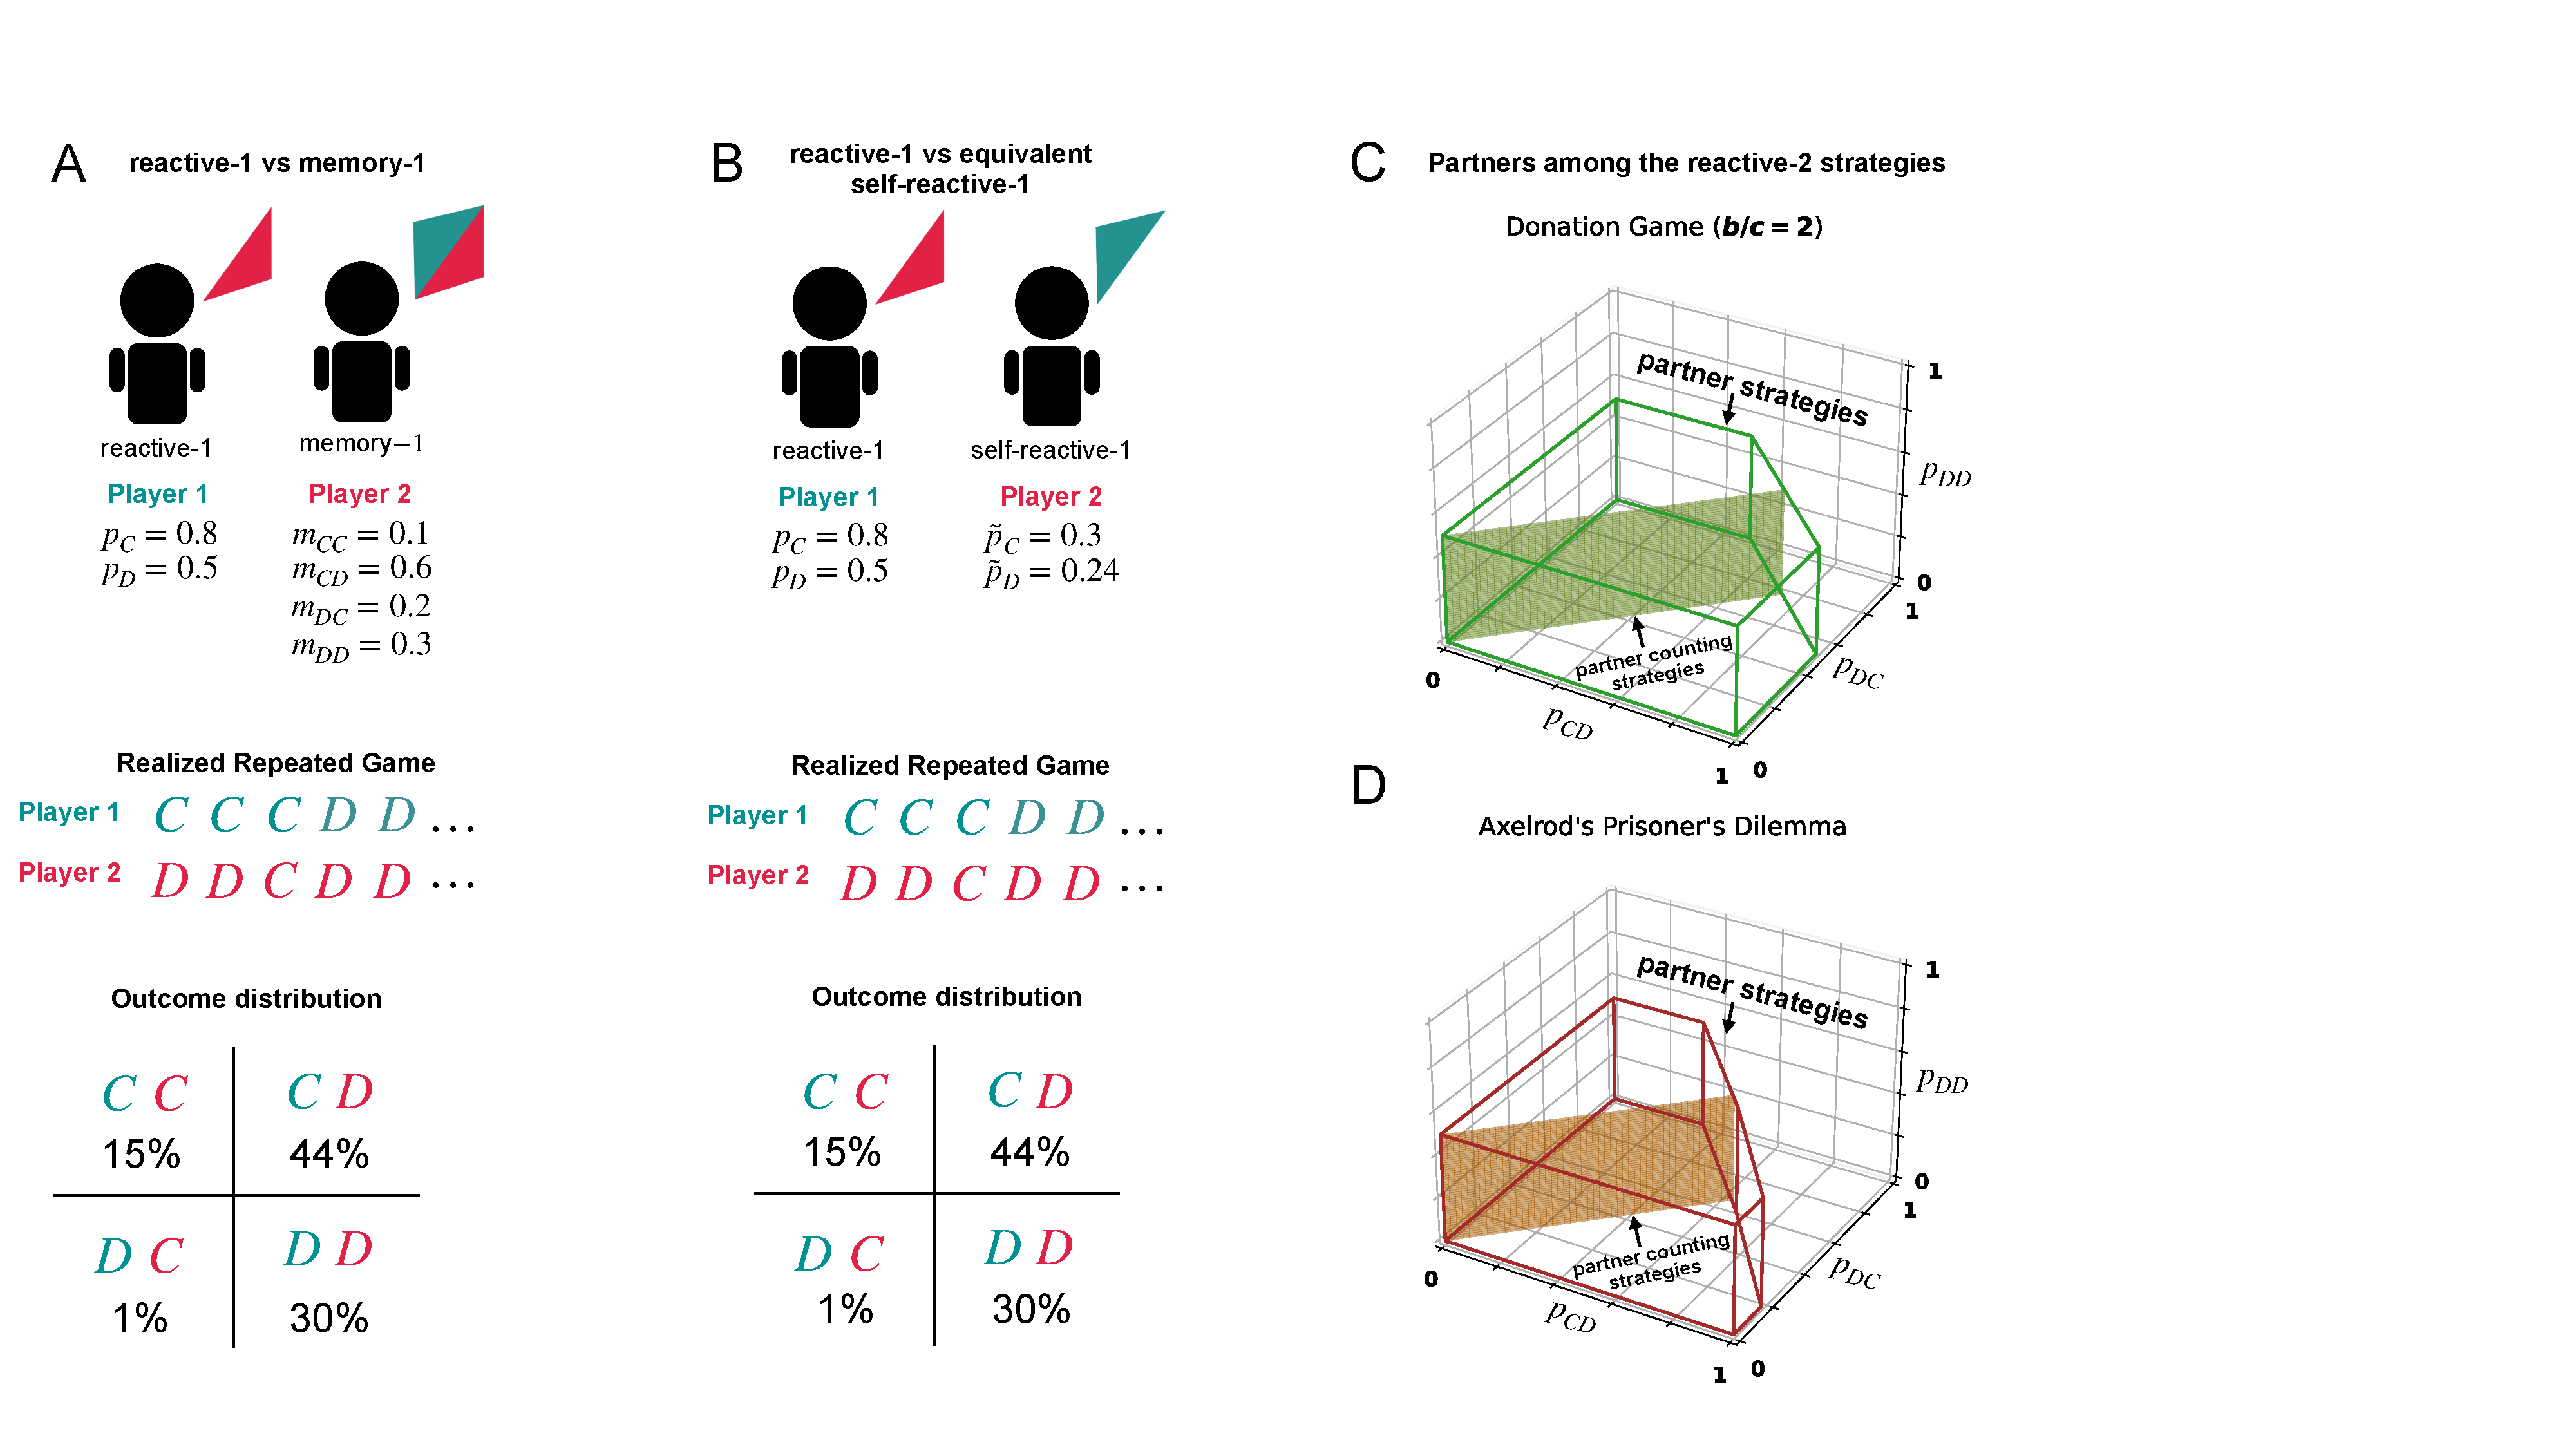
\includegraphics[width=\textwidth]{figures/conceptual_figure_results.pdf}
  \caption{
  \textbf{Characterizing the partners among the reactive-$n$ strategies.} 
{\bf A,B,} To characterize the reactive-$n$ partner strategies, we prove the following result. 
Suppose the focal player adopts a reactive-$n$ strategy. 
Then, for any strategy of the opponent (with arbitrary memory), one can find an associated self-reactive-$n$ strategy that yields the same payoffs. 
Here, we show an example where player~1 uses a reactive-1 strategy against player~2 with a memory-1 strategy. 
Our result implies that can switch to a well-defined self-reactive-1 strategy. 
This switch leaves the outcome distribution unchanged.
In both cases, players are equally likely to experience mutual cooperation, unilateral cooperation, or mutual defection in the long run. 
\textbf{C,} Based on this insight, we can explicitly characterize the reactive-2 partner strategies (with $p_{CC}\!=\!1$). 
Here, we represent the corresponding conditions~\eqref{eq:two_bit_conditions} for a donation game with $b/c\!=\!2$. 
Among the reactive-2 strategies, the counting strategies correspond to the subset with $p_{CD}\!=\!p_{DC}$. 
Counting strategies only depend on how often the co-player cooperated in the past, not on the timing of cooperation.
\textbf{D,} Similarly, we can also characterize the reactive-2 partner strategies for the general prisoner's dilemma. 
Here, we use the values of Axelrod~\citep{axelrod:AAAS:1981}.
}\label{fig:conceptual_figure_results}
\end{figure}

\begin{figure}[t]
  \centering
  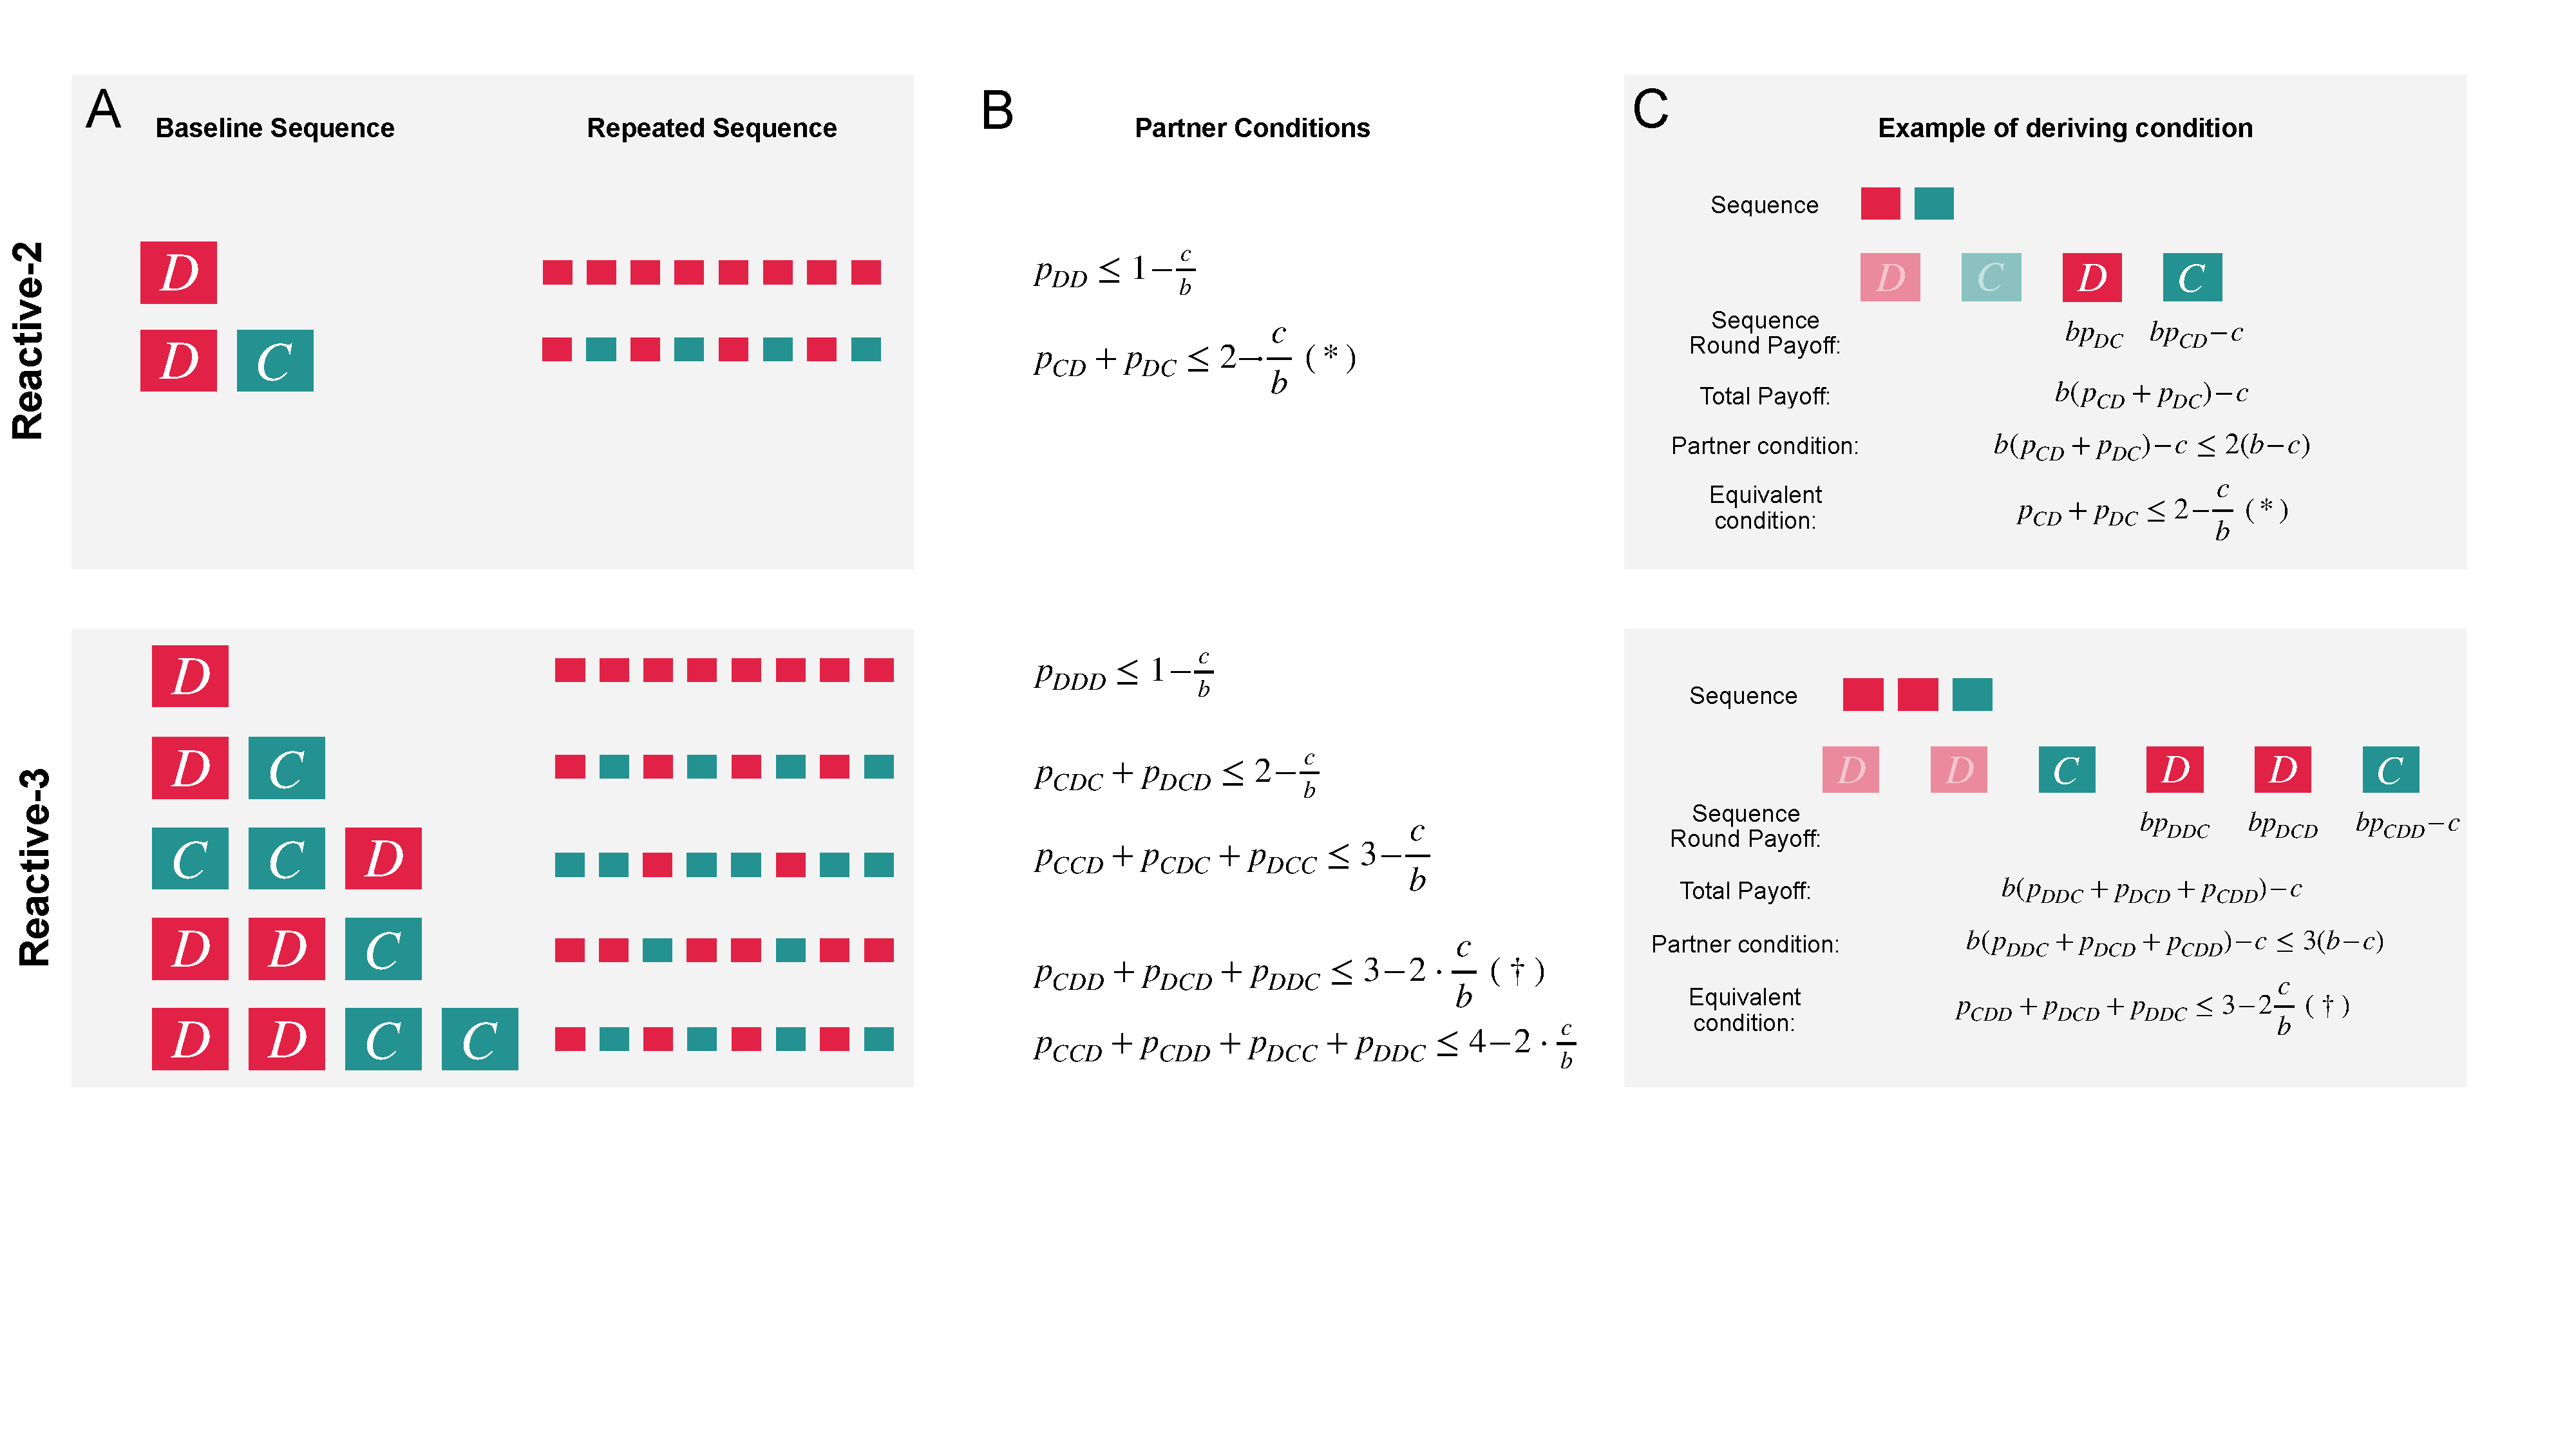
\includegraphics[width=\textwidth]{figures/conceptual_figure_conditions.pdf}
  \caption{
  \textbf{Conditions for partners among reactive-$2$ and reactive-$3$ strategies.}
  {\bf A, B,} Within the set of pure self-reactive strategies, there are certain
  strategies where the way they behave can be described as playing a unique
  sequence. Since their action does not depend on the co-player's history, the
  strategy plays this sequence indefinitely. For example, in the case of \(n=2\),
  the pure self-reactive strategy \(\mathbf{\tilde{p}}=(0, 1)\), which alternates,
  can be described as playing the sequence \((D, C)\).
  {\bf C,} We have proven that to characterize reactive-\(n\) partner strategies, one only
  needs to check deviations towards self-reactive-\(n\) strategies. Thus, for a
  nice reactive strategy \(p\) to be a partner, it is necessary that none of these
  sequence-playing self-reactive strategies can achieve a higher payoff against
  \(p\) than \(p\) does against itself. The conditions of partner strategies, for
  \(n=2\), and \(n=3\), respectively for each of the sequences in panel {\bf
  A}, are shown in panel {\bf C}. These conditions are necessary, but
  furthermore, we have shown that these are also sufficient conditions (see
  \SI).
  {\bf D,} To derive the conditions, we need to consider the payoff that a sequence player
  achieves against a reactive strategy. In the top panel of panel {\bf D}, we
  illustrate an example for \(n=2\), against \(\mathbf{p} = (1, p_{CD}, p_{DC},
  p_{DD})\) and the sequence \((D, C)\). In the third turn, the sequence player
  receives a benefit \(b\) with a probability of \(p_{DC}\), and no cost since the
  sequence player did not cooperate. In the fourth turn, the player receives
  \(p_{DC} \cdot b - c\), and thereafter these two payoffs are repeated forever.
  Thus, the total payoff of the sequence player with memory two is given by what
  they receive every two turns, which is \(p_{DC} \cdot b - c\). This payoff needs
  to be smaller or equal than what a partner strategy achieves against another
  nice strategy, which is \(2(b\!-\!c)\).
  In the bottom panel of panel {\bf D}, we illustrate an example for $n=3$.
  }\label{fig:conceptual_figure_conditions}
\end{figure}


\begin{figure}[t]
  \centering
  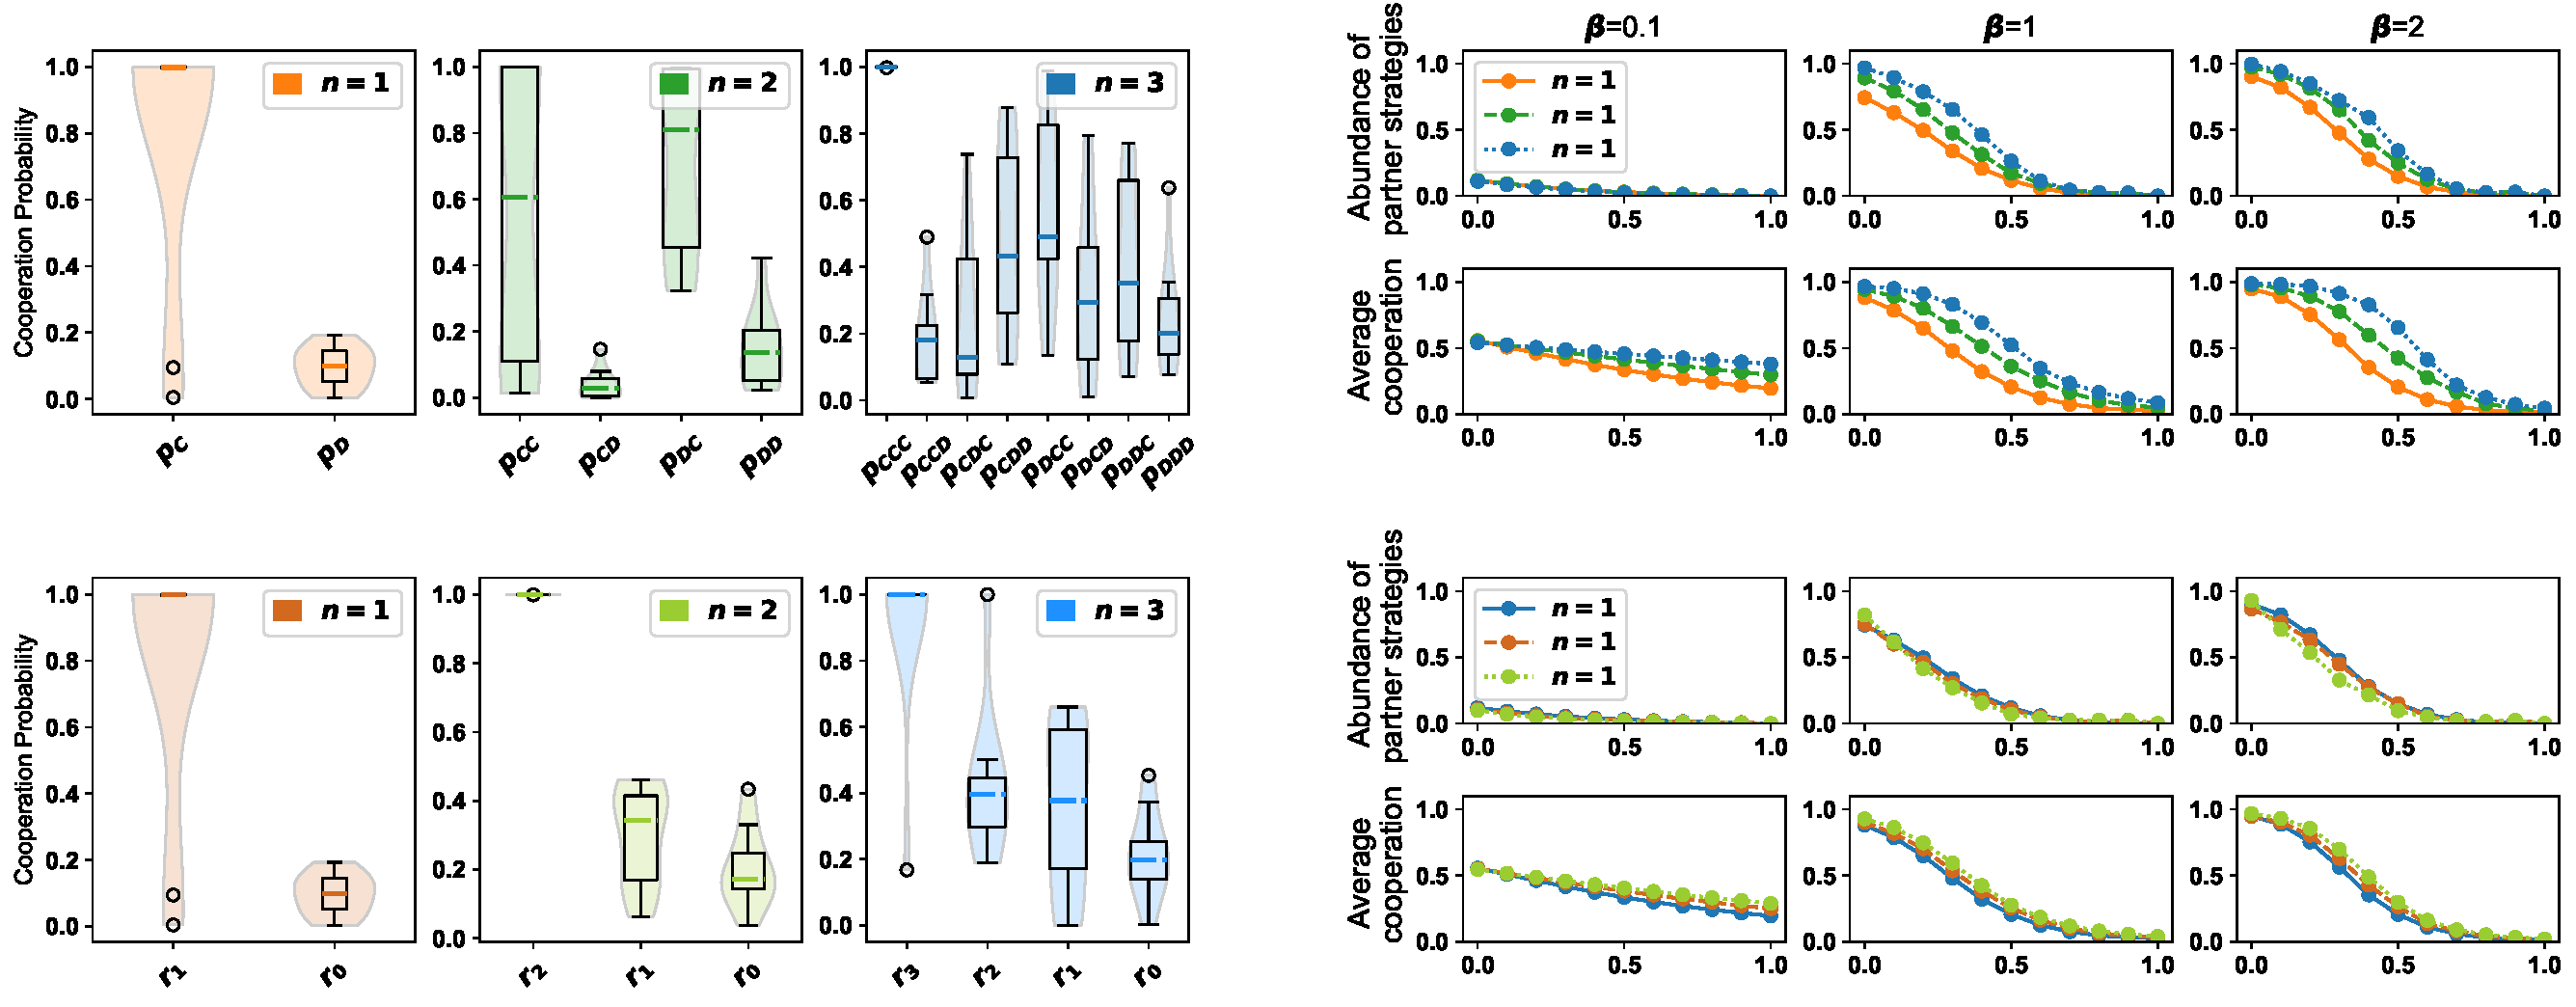
\includegraphics[width=\textwidth]{figures/abundant_strategies.pdf}
  \caption{\textbf{Evolutionary dynamics of reactive-$n$ strategies.}
  To explore the evolutionary dynamics among reactive-$n$ strategies, we run simulations based on the
  method of Imhof and Nowak~\cite{imhof:royal:2010}. 
  This method assumes rare mutations. 
  Every time a mutant strategy appears, it goes extinct or fixes before the arrival of the next mutant strategy. 
  {\bf A,B,} We run ten independent simulations for reactive-$n$ strategies and for reactive-$n$ counting strategies. 
  For each simulation, we record the most abundant strategy (the strategy that resisted most mutants). 
  The respective average cooperation probabilities are in line with the conditions for partner strategies. 
  {\bf C,D,} With additional simulations, we explore the average abundance of partner strategies and the population's average cooperation rate. 
For a given resident strategy to be classified as a partner by our simulation, it needs to satisfy all inequalities in the respective definition of partner strategies. 
In addition, it needs to cooperate after full cooperation with a probability of at least 95\%.  
For all considered parameter values, we only observe high cooperation rates when partner strategies evolve. 
Simulations are based on a donation game with \(b\!=\!1\),  \(c\!=\!0.5\), a selection strength $\beta\!=\!1$
and a population size $N\!=\!100$, unless noted otherwise. For $n$ equal to 1 and 2, simulations are run for \(T\!=\! 10 ^ 7\) time steps. For $n\!=\!3$ we use \(T\!=\! 2 \!\cdot\!10 ^ 7\) time steps.
}\label{fig:evolutionary_results}
\end{figure}


\end{document}




